% Name: Similar triangles
% Description: Triangle DEF is triangle ABC scaled by 3/2: the angles match, and each side is 1.5 times the side it corresponds to.
% Tags: similar triangles, scale factor, ratio, angles

\usetikzlibrary{angles}

\begin{tikzpicture}[thick, every node/.style={font=\small}, mark/.style={draw, angle radius=#1}]
  % Sides 4, 5, and 6 on a base of 6: the apex is at (27/12, sqrt(16 - (27/12)^2)) = (2.25, 3.3072)
  \begin{scope}[scale=0.6]
    \coordinate[label=below left:$B$] (B) at (0,0);
    \coordinate[label=below right:$C$] (C) at (6,0);
    \coordinate[label=above:$A$] (A) at (2.25,3.3072);
    \draw (A) -- node[above left] {$4$} (B) -- node[below] {$6$} (C) -- node[above right] {$5$} cycle;
    \pic[mark=5mm] {angle=C--B--A};
    \pic[mark=4mm] {angle=A--C--B}; \pic[mark=5mm] {angle=A--C--B};
    \pic[mark=3mm] {angle=B--A--C}; \pic[mark=4mm] {angle=B--A--C}; \pic[mark=5mm] {angle=B--A--C};
  \end{scope}
  \begin{scope}[xshift=5cm, scale=0.9]
    \coordinate[label=below left:$E$] (E) at (0,0);
    \coordinate[label=below right:$F$] (F) at (6,0);
    \coordinate[label=above:$D$] (D) at (2.25,3.3072);
    \draw (D) -- node[above left] {$6$} (E) -- node[below] {$9$} (F) -- node[above right] {$7.5$} cycle;
    \pic[mark=5mm] {angle=F--E--D};
    \pic[mark=4mm] {angle=D--F--E}; \pic[mark=5mm] {angle=D--F--E};
    \pic[mark=3mm] {angle=E--D--F}; \pic[mark=4mm] {angle=E--D--F}; \pic[mark=5mm] {angle=E--D--F};
  \end{scope}
  \node at (5.5,-1.2) {$\dfrac{DE}{AB} = \dfrac{EF}{BC} = \dfrac{FD}{CA} = \dfrac{3}{2}$};
\end{tikzpicture}
